%
\section{Automatische Statische Analyse}
Zur statischen Analyse von C\# Programmen stehen eine Reihen an Werkzeugen zur Verfügung. Einerseits gibt es in die Entwicklungsumgebung integrierte Werkzeuge wie \emph{NDepend}, \emph{ReSharper} und das von Visual Studio bereitgestellt Tool, andererseits eigenständige Programme wie \emph{Gendarme} und \emph{SourceMonitor}.

\subsection{Visual Studio Tools}
Visual Studio analysiert Code, erstellt dabei Quelltextmetriken und kann zum Beispiel Code-Clone identifizieren. Alle bereitgestellten Werkzeuge sind einfach gehalten. Einerseits wirkt die Entwicklungsumgebung dadurch nicht überladen, andererseits fehlt einiges an Komfort bei der Entwicklung.

\subsubsection{Quelltextmetriken}
Standardmäßig bietet Visual Studio einige Metriken an. Es listet die Ergebnis in der Hierarchie, welche durch den Quelltext gegeben ist. Alle weiteren Werkzeuge bieten diese Funktion ebenfalls an. Deswegen wird es der Vollständigkeit halber erwähnt, dass Visual Studio selbstständig ebenfalls Quelltextmetriken analysieren kann.

Die einzige interessante Metrik ist die Vererbungsebenen jeder Klasse. Auf Basis dieser Metrik lassen sich Klassen identifizieren, die eine tiefe Hierarchie aufspannen. Basisklassen solcher Vererbungshierarchien müssen besonders gut getestet werden, damit sich Fehler dieser Klassen nicht auf alle anderen auswirken. In Extremfällen kann ein hoher Wert auf einen Fehler in der Architektur des Programmes hinweisen. In C\# Essentials liegt der Wert in einem normalen Bereich zwischen 1 und 3, es gibt keine Ausreißer nach oben oder unten.

\subsubsection{Code-Clone}
Die Suche nach Quelltextduplikaten bietet von allen gefundenen Werkzeugen nur Visual Studio an. Abbildung~\ref{fig:vs-code-clones} zeigt die in C\# Essentials gefundenen Quelltextduplikate. Bei beiden Stellen ist sich Visual Studio nicht sicher, ob es sich um ein Duplikat handelt. Das Listing~\ref{lst:code-VSMediumDuplicate} zeigt den Quelltextabschnitt, den Visual Studio als \enquote{Medium Match} bezeichnet. Die beiden \texttt{case} Statements sind Teil eines \texttt{switch} mit drei weiteren Fällen. Zwar kann es nützlich sein solche Duplikate zu finden, um die Architektur eines Programms verbessern, jedoch ist es abhängig vom betrachteten Quelltext nicht immer sinnvoll Änderungen vorzunehmen. In dem Beispiel, betrachtet man nur die beiden gezeigten Statements erscheint es sinnvoll, den Quelltext anzupassen. Erweitert man den betrachteten Bereich auf alle \texttt{case} Statements ist es schwerer mit einem sauberen Ansatz den Quelltext zu verbessern.

Im Beispiel war es nicht möglich aus dem Analyseergebnis einen direkten Nutzen zu ziehen. Insgesamt ist es wichtig ein solches Werkzeug zur Verfügung zu haben, schließlich möchte man Quelltext nur ungern doppelt schreiben, da es erstens unnötige Arbeit ist und zweitens die Architektur des Programms beeinträchtigt.

\begin{figure}[!ht]
	\centering
	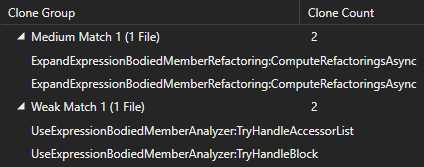
\includegraphics[width=0.8\textwidth]{images/vs-code-clones.png}
	\caption{Code Clones in C\# Essentials}
	\vspace{0.1cm}
	Visual Studio sortiert die gefundenen Stellen nach\\ der Wahrscheinlichkeit, ob es wirklich ein Duplikat ist.
	\label{fig:vs-code-clones}
\end{figure}

\begin{minipage}{\textwidth}
	\begin{lstlisting}[caption={Visual Studio Medium Dublikat},
	label={lst:code-VSMediumDuplicate}]
	case SyntaxKind.MethodDeclaration:
		var methodDeclaration = (MethodDeclarationSyntax)declaration;
		if (methodDeclaration.ExpressionBody != null)
		{
			context.RegisterRefactoring(
			CodeAction.Create(
			"Expand expression-bodied member",
			c => HandleMethodDeclaration(methodDeclaration, context.Document, c)));
		}
		
		break;
		
	case SyntaxKind.OperatorDeclaration:
		var operatorDeclaration = (OperatorDeclarationSyntax)declaration;
		if (operatorDeclaration.ExpressionBody != null)
		{
			context.RegisterRefactoring(
			CodeAction.Create(
			"Expand expression-bodied member",
			c => HandleOperatorDeclaration(operatorDeclaration, context.Document, c)));
		}
		break;
	\end{lstlisting}
\end{minipage}

\subsection{NDepend}
\emph{NDepend} führt statischen Analysen von Projekten durch, erstellt dabei Softwarelandkarten, Codemetriken und überprüft ob Quelltextregel eingehalten werden.~\cite{ndepend} Auf der \enquote{Dashboard} genannten Übersicht erstellt \emph{NDepend} eine Zusammenfassung aller Analysen. 

\subsubsection{Quelltextregel}
NDepend ermittelt in C\# Essentials insgesamt 37 verletzte Regeln, dabei finden 150 Regeln Anwendung. An dieser Stelle soll nur auf die als kritisch markierten Regeln eingegangen werden. 3 kritische Regelverletzungen ermittelt NDepend: Methods too complex (2), Potenially dead Methods (6), Potentially dead Types (6). Weitere verletzte Regeln sind in erster Linie nicht eingehaltene Namenskonventionen, Sichtbarkeiten und Design Schwächen. Um potentielle Fehler zu finden, werden im Folgenden kritische Stellen genauer analysiert.

\paragraph{Methods too complex}
Auf diese gefundene Regelverletzung wird nur kurz eingegangen, weil sie auf Quelltextmetriken basiert, die später im Abschnitt~\ref{sec:nd-code-metrics} betrachtet werden.

Das wichtigste Detail, welches bei der Verwendung von \emph{NDepend} auffiel, ist , dass die Klasse \texttt{ConvertToInterpolatedStringRefactoring} die in Abbildung~\ref{fig:nd-methode-too-complex} gezeigte Methode \texttt{MoveNext} gar nicht besitzt. Schaut man sich den Quelltext an, stellt man fest: \emph{NDepend} hat eigentlich die Methode \texttt{ComputeRefactoringsAsync} gefunden.

Die Ursache für den falsch identifizierten Namen liegt in der Implementierung des \texttt{async} Schlüsselworts in C\#. Als asynchron deklarierte Methoden werden in C\# als Zustandsautomat modelliert.~\cite{csharp-async} Die Methode \texttt{ComputeRefactoringsAsync} ist dabei nur einer von vielen Zuständen innerhalb der Methode \texttt{MoveNext}. Deshalb schafft es \emph{NDepend} nicht sie richtig zu identifizieren. Die als zu komplex identifizierten Methoden werden im Abschnitt Testen genauer analysiert.

Kriterien für eine als zu komplex eingestufte Methode sind eine Nesting Depth größer vier, eine Cyclomatic Complexity über 20 oder eine IL Cyclomatic Complexity über 40.~\cite{nd-cc-criteria}

\begin{figure}[!ht]
	\centering
	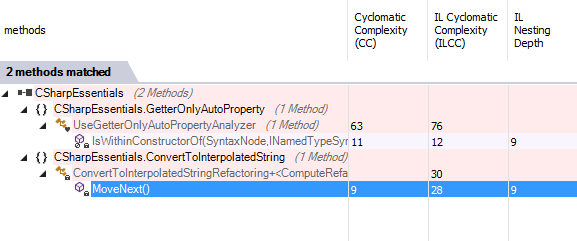
\includegraphics[width=\textwidth]{images/methode-too-complex.png}
	\caption{Methods too complex}
	\vspace{0.1cm}
	Methoden, welche NDepend als zu komplex einstuft.
	\label{fig:nd-methode-too-complex}
\end{figure}

\paragraph{Potentially dead Methods} In C\# Essentials findet \emph{NDepend} sechs mögliche Stellen, an denen Quelltext nicht ausgeführt wird. In Abbildung~\ref{fig:dead-methods} sieht man die gefundenen Stellen. Bei allen handelt es sich um nicht aufgerufenen Konstruktoren. Jedoch ist keine der gefundenen Methoden ein Konstruktor. Ähnlich der \texttt{MoveNext} Methode diagnostiziert eine falsche Methode. Alle identifizierten Methoden sind statisch deklariert, was scheinbar die Fehlerquelle der falschen Namen ist. Jedoch konnte keine Ursache für dieses Fehlverhalten gefunden werden. Außerdem sind alle Funde mindestens einmal im Quelltext referenziert und somit verwendet worden.

\begin{figure}[!ht]
\centering
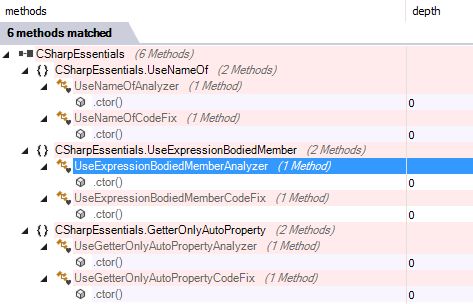
\includegraphics[width=0.9\textwidth]{images/dead-methods.png}
\caption{Potentially dead Methods}
\vspace{0.1cm}
Von NDepend gefundener wahrscheinlich nicht aufgerufener Quelltext
\label{fig:dead-methods}
\end{figure}

\subsubsection{Quelltextmetriken}
\label{sec:nd-code-metrics}
Mit Hilfe des \enquote{Code Metrics View} visualisiert \emph{NDepend} Quelltextmetriken. Auflösungen von Assembly über Namespaces bis Methoden stehen zur Auswahl. In größeren System, welche aus mehren Assemblies bestehen, möchte man nach kritischen Teilprogrammen suchen. Mit knapp über 1000 Quelltextzeilen und nur einer Assembly in C\# Essentials ist die Auflösung nach Methoden am sinnvollsten. IL Nesting Depth, Cyclomatic Complexity und IL Cyclomatic Complexity erzeugen die in den Abbildungen~\ref{fig:nd-il-nesting-depth},~\ref{fig:nd-cyclomatic-complexity} und ~\ref{fig:nd-il-cyclomatic-complexity} dargestellten Code Metric Views. Metriken mit einem führenden \enquote{IL} werden auf Basis der \enquote{Intermediate Language} erstellt. Mehr zur \emph{IL} in Abschnitt \ref{sec:gendarme}. Die Programmierer von NDepend definieren jede Metrik und geben zusätzlich einen empfohlenen Maximalwert an.~\cite{ndepend-metrics}

Die \emph{Cyclomatic Complexity}, welche auch \enquote{McCabe-Metrik} genannt wird, gibt an wie viele binäre Verzweigungen in einem Programmabschnitt vorliegen. Eine solche Verzweigung wird zum Beispiel durch \texttt{if} Statements erzeugt. ~\cite{mccabe} McCabe empfiehlt der Wert sollte niemals höher als 10 liegen. Durch einen geringen Wert, lassen sich Methoden besser testen, weil die Anzahl der entstandenen Pfade kleiner ist.

\emph{NDepend} unterscheidet \emph{Cyclomatic Complexity} und \emph{IL Cyclomatic Complexity}, weil einige Statements in der Intermediate Language aufgesplittet werden. Eine \texttt{foreach} Schleife resultiert zum Beispiel in 3 Pfaden eine \texttt{for} Schleife nur in 2. Folglich ist der IL Wert etwas höher als der normale.

Der praktische Nutzen dieser Unterscheidung ist diskutabel, weil beim Testen das Verhalten des Programmes selbst verifiziert werden soll und nicht die korrekte Übersetzung in die Intermediate Language. Für einen wirklichen Nutzen muss ein Fall vorliegen, bei dem zwei Schreibweisen eines Programmes zu unterschiedlichen Aussagen in der Intermediate Lanuage führen.

Die graphischen Analysen von C\# Essentials weisen sowohl auf eine hohe Verschachtlungstiefe (Abbildung~\ref{fig:nd-il-nesting-depth}), als auch eine hohe McCabe-Metrik (Abbildungen~\ref{fig:nd-cyclomatic-complexity} und~\ref{fig:nd-il-cyclomatic-complexity}) der Methode \texttt{UpdateExpression} in der Klasse \texttt{UseGetterOnlyAutoPropertyAnalyzer} hin. Damit liefert \emph{NDepend} einen Hinweis dafür, dass diese Methode eine hohe Priorität beim Testen haben sollte.

\begin{figure}[!ht]
	\centering
	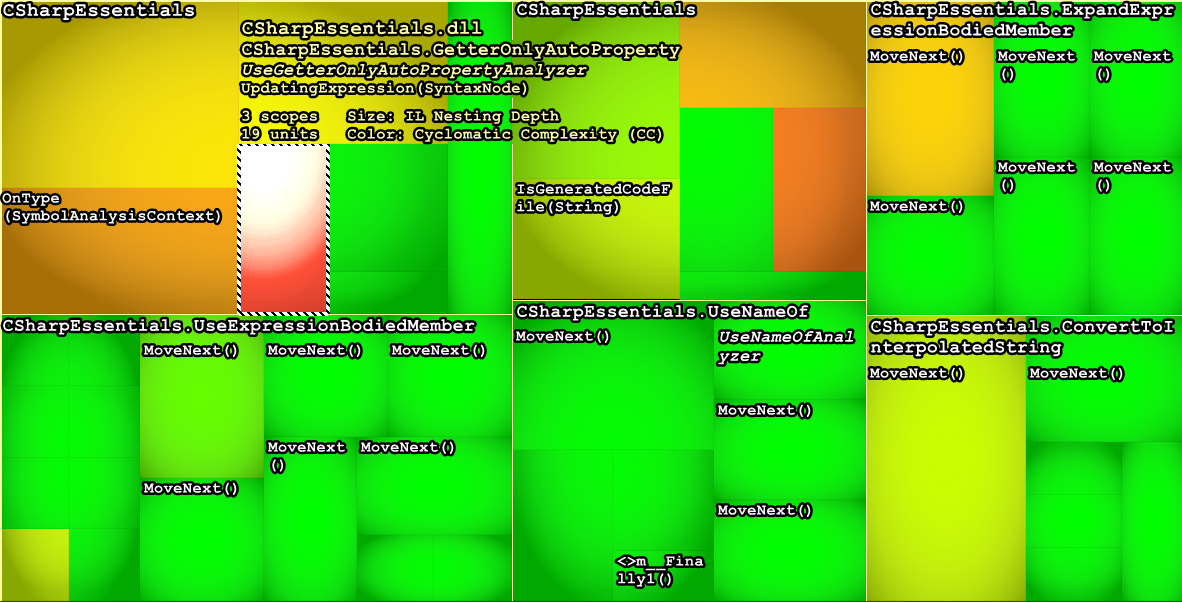
\includegraphics[width=0.8\textwidth]{images/nd-il-nesting-depth.png}
	\caption{IL Nesting Depth}
	\vspace{0.1cm}
	\label{fig:nd-il-nesting-depth}
	Die Methode \texttt{UpdateExpression weist eine sehr \\ hohe Verschachtelungstiefe auf. \\ Andere Methoden besitzen ebenfalls hohe Werte.}
\end{figure}

\begin{figure}[!ht]
	\centering
	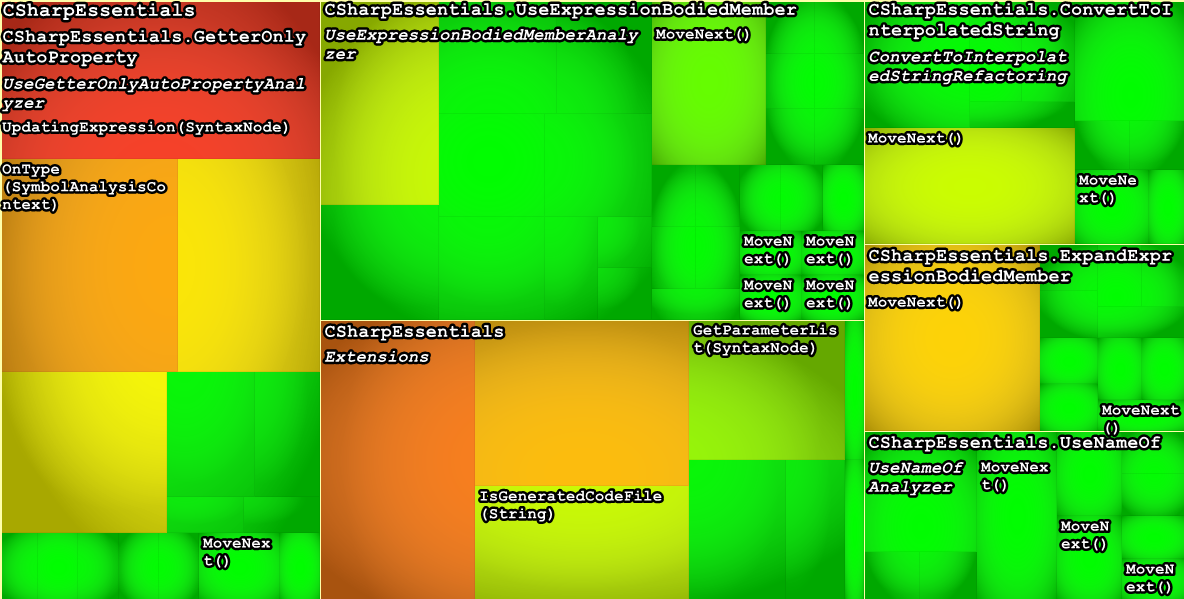
\includegraphics[width=0.8\textwidth]{images/nd-cyclomatic-complexity.png}
	\caption{Cyclomatic Complexity}
	\vspace{0.1cm}
	Neben \texttt{UpdateExpression} gibt es zwei\\ weitere Methoden mit hoher Komplexität.
	\label{fig:nd-cyclomatic-complexity}
\end{figure}

\begin{figure}[!ht]
	\centering
	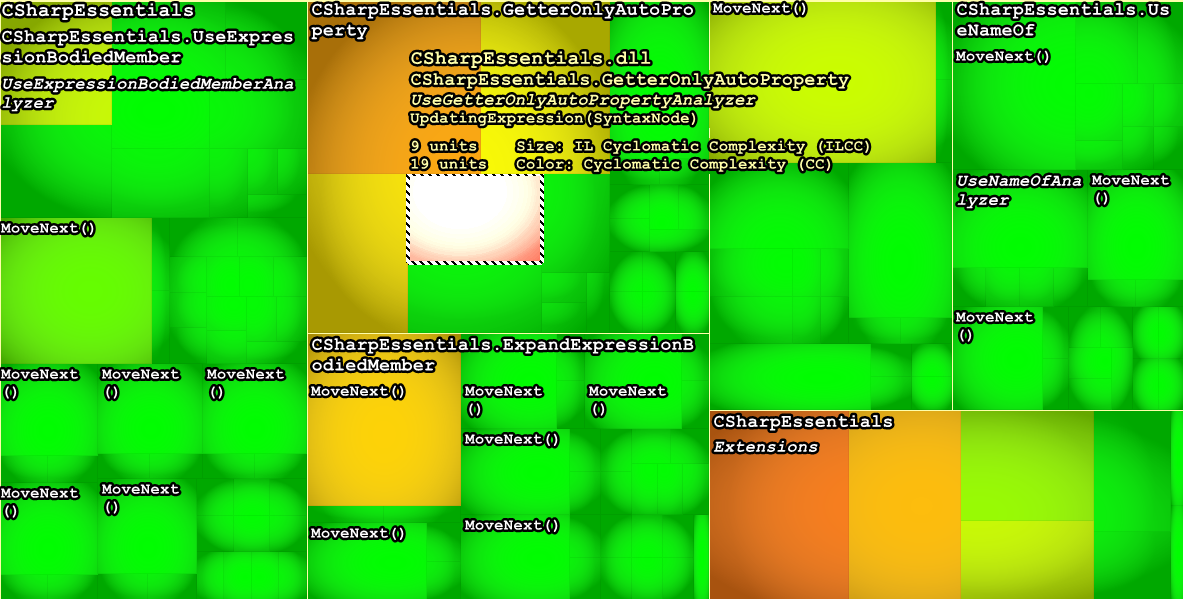
\includegraphics[width=0.8\textwidth]{images/nd-il-cyclomatic-complexity.png}
	\caption{IL Cyclomatic Complexity}
	\vspace{0.1cm}
	Trotzdem die IL Werte eigentlich größer sind, \\
	sieht diese Ansicht besser aus als die in \\ Abbildung~\ref{fig:nd-cyclomatic-complexity} gezeigte.
	\label{fig:nd-il-cyclomatic-complexity}
\end{figure}

\subsection{ReSharper}
Mit \emph{ReSharper} bietet JetBrains ein Werkzeug zur statischen Analyse für Visual Studio an.~\cite{resharper} \emph{ReSharpers} größter Vorteil ist, dass es - ähnlich wie C\# Essentials - die Visual Studio Funktion für Quelltextverbesserungsvorschläge nutzt. Abbildung~\ref{fig:rsharper-code-metric-inline} weist, ähnlich wie \emph{NDepend}, auf eine hohe Cyclomatic Complexity der Methode \texttt{UpdateExpression} hin. Entsprechend den von \emph{ReSharper} berechneten Werten sollte \emph{NDepend} auch diese Methode als zu komplex identifizieren. Zusätzlich findet es selbst die in der Code Metric View sehr hohe Komplexitätswerte. An dieser Stelle liefert \emph{ReSharper} die eindeutigeren und somit besseren Ergebnisse.

\begin{figure}[!ht]
	\centering
	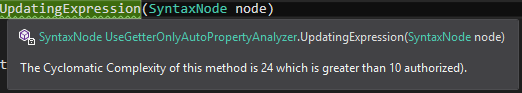
\includegraphics[width=0.8\textwidth]{images/rsharper-code-metric-inline.png}
	\caption{ReSharper Quelltextmetriken in Visual Studio IntelliSense}
	\vspace{0.1cm}
	\emph{ReSharper} gibt beim Klick auf eine Methode \\
	direktes Feedback zu hohen Quelltextmetrikwerten 
	\label{fig:rsharper-code-metric-inline}
\end{figure}

\subsection{Gendarme}
\label{sec:gendarme}
Gendarme analysiert Programme und Bibliotheken, welche in den verschiedenen .NET Sprachen geschrieben wurden. Dafür benötigt Gendarme eine kompilierte Assembly, weil es nicht den C\# statisch analysiert, sondern ein daraus erzeugte Spracheformat: Das ECMA CLI~\footnote{European Computer Manufacturers Association Common Language Infrastructure} Format. Die CIL wird mit Hilfe von der Bibliothek Cecil analysiert.~\cite{cecil}
 
\paragraph{ECMA CLI} Die \enquote{Common Language Infrastructure} ist ein standardisiertes Sprachformat, welches eine Ausführung mehrerer Sprachen in einer Laufzeitumgebung ermöglicht. Mit diesem Standard setzt Microsoft zum Beispiel die Interoperabilität der .NET Sprachen C\# und F\# um. ~\cite{ecma}

\vspace{0.2cm}

\emph{Gendarme} generiert auf Basis dieser Analyse Berichte. Sie können als HTML-Datei exportiert werden. Insgesamt konnten wir aus den Analysen von \emph{Gendarme} keine nützlichen Hinweise gewinnen. Der einzige mit hoher Dringlichkeit eingeschätzte Fehler, ist ein fehlendes Attribut der Assembly-Datei. Dieses weist, wenn verwendet, darauf hin, dass die Klassen mit aufgrund der Intermediate Language auch in anderen .NET Sprachen verwendet werden können. Andere gefundene Fehler weisen lediglich darauf hin, dass die Namespaces in C\# Essentials aus zu wenig Klassen bestehen. 

Der Vorteil von \emph{Gendarme} ist, dass man vor der Analyse eine gewünschte Fehler- und Sicherheitstoleranz definieren kann. So lassen sich Programme nur auf kritische, oder alle möglichen Fehler untersuchen. Zusätzlich kann man definieren, wie sicher sich \emph{Gendarme} sein muss, damit es eine mögliche Fehlerquelle als Fehler meldet. Für die Verifizierung eines Programmes, lässt sich hier absolute Sicherheit konfigurieren. In C\# Essentials werden mit dieser Einstellung 4 Fehler gefunden. Zum einen das bereits erwähnte, fehlende Attribut, zum anderen die zu kleinen Namespaces.

\subsection{SourceMonitor}
Der Fokus von \emph{Source Monitor} liegt auf der Analyse von Quelltextmetriken. Es bietet die Möglichkeit einzelne Checkpoints für bestimmte Teile des Programmes zu erstellen und miteinander zu vergleichen. Abbildung~\ref{fig:source-monitor-avg-complexity} zeigt den Vergleich der kompletten Quelltextbasis (Tests, Hauptprogramm) mit dem Hauptprogramm und der Klasse \texttt{UseGetterOnlyAutoPropertyAnalyzer}, welche die höchsten Werte in \enquote{Avg. Depth} und \enquote{Avg. Complexity} aufweist.

Die Statistik zeigt: Die hohe Komplexität geht einher mit einer hohen Anzahl an Statements in der Klasse und vielen Statements pro Methode. Mit Hilfe einer einfachen Visualisierung ist es möglich innerhalb weniger Minuten die kritischen Stellen eines Programmes zu identifizieren. Auf diese Weise ist es leichter zu bestimmen, welche Programmteile besonderen Fokus in der Phase des Testens haben sollten.

\begin{figure}[!ht]
	\centering
	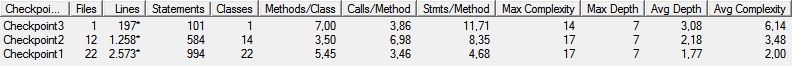
\includegraphics[width=\textwidth]{images/source-monitor-avg-complexity.png}
	\caption{Source Monitor Quelltextmetriken}
	\vspace{0.1cm}
	Checkpoint 1 - gesamte Quelltextbasis, Checkpoint 2 - Hauptprogramm,\\ Checkpoint 3 - die Klasse \texttt{UseGetterOnlyAutoPropertyAnalyser}
	\label{fig:source-monitor-avg-complexity}
\end{figure}

\subsubsection{Kiviat-Chart}
\enquote{Kiviat-Charts} sind eine Alternative zu den mit \emph{NDepend} vorgestellten Code-Metric-Views. Sie visualisieren alle Statistiken zum Quelltext auf einen Blick und man muss nicht zwischen einzelnen Ansichten wechseln, wie in Abbildung~\ref{fig:source-monitor-kiviat-chart} gezeigt. Nachteil dieser Ansicht ist die nicht skalierbare Auflösung.

Mit Kiviat-Charts lassen sich Quelltextmetriken bezüglich bestimmter Minimal- und Maximalwerte veranschaulichen.~\cite{kiviat} Abbildung~\ref{fig:source-monitor-kiviat-chart} zeigt zwei Charts, die aus dem Quelltext von C\# Essentials generiert wurden. Alle Metriken in grünen Bereich, liegen innerhalb der empfohlenen Werte. Ähnlich wie die bereits vorgestellten Werkzeuge weist auch \emph{Source Monitor} auf eine zu hohe Komplexität hin. Die Klasse \texttt{UseGetterOnlyAutoProperty} sticht hier wieder negativ hervor.

Zusätzlich weist \emph{Source Monitor} darauf hin, dass die Anzahl der dokumentierten Klassen und Methoden zu gering ausfällt. Im allgemeinen lassen sich für Dokumentation keine einheitlich festgelegten Werte finden, deshalb kann man diesen Wert als Hinweis interpretieren. Es lassen sich aus ihm keine direkten Schlüsse auf die Qualität des Quelltextes ziehen. Bei öffentlichen Schnittstellen sollte man den Wert dennoch beachten.

\begin{figure}[!ht]
	\centering
	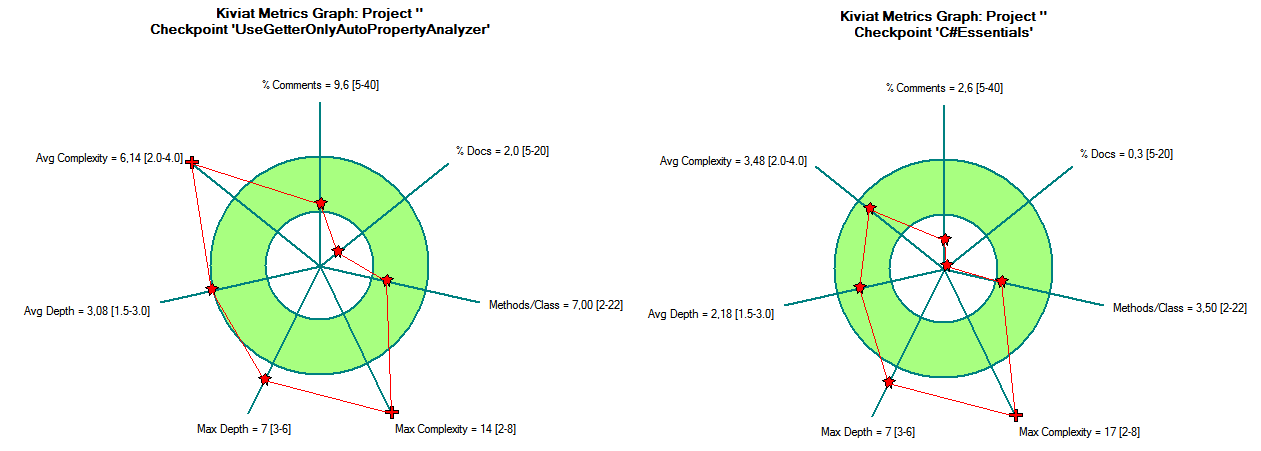
\includegraphics[width=\textwidth]{images/source-monitor-kiviat-chart.png}
	\caption{Kiviat-Charts}
	\vspace{0.1cm}
	Im Vergleich die Klasse \texttt{UseGetterOnlyAutoPropertyAnalyzer} (links) \\ und das gesamte Projekt (rechts).
	\label{fig:source-monitor-kiviat-chart}
\end{figure}

\newpage

\subsubsection{Quelltextmetriken im Verlauf}
\emph{Source Monitor} bietet eine weitere Funktion an: Es lässt sich ein Verlauf der Quelltextmetriken über einen bestimmten Zeitraum analysieren. Auf diese Weise kann man direkten Nutzen aus den Metriken ziehen - übersteigt ein Wert einen für ein Projekt festgelegten Schwellwert, kann die Architektur angepasst werden, um den Ansprüchen wieder zu entsprechen. Weiterhin ist es denkbar, eine Analyse durchzuführen, ab welchem Zeitpunkt in der Projektdurchführung die Quelltextqualität Veränderungen erfahren hat. \emph{C\# Essentials} ist ein fertiggestelltes Projekt, welches wir selber nicht entwickelt haben, deshalb wird in Abbildung~\ref{fig:source-monitor-time-metric-chart} ein aus dem Git-Repository erzeugter Verlauf gezeigt.

\begin{figure}[!ht]
	\centering
	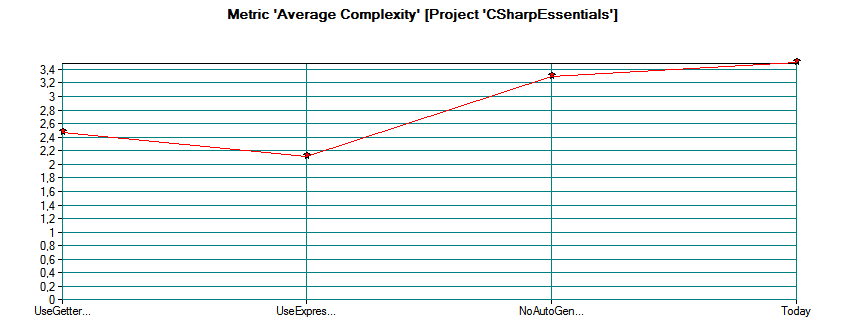
\includegraphics[width=\textwidth]{images/source-monitor-avg-complexity-over-time.png}
	\caption{Average Complexity des Projekts im Zeitverlauf}
	\vspace{0.1cm}
	Betrachtet wird die durchschnittlich Komplexität \\ des Projektes zu Zeitpunkten, an denen relativ \\ zur vorhandenen Menge viel Quelltext hinzugefügt wurde.
	\label{fig:source-monitor-time-metric-chart}
\end{figure}

\newpage

\subsection{ASA Werkzeuge - Ein Vergleich}
Tools wie \emph{NDepend} und \emph{ReSharper} stellen eine große Menge an Funktionen bereit, welche die ASA von C\# Programmen und das Schreiben von Tests erleichtern. Die Fehler in den Analysen von \emph{NDepend} sind störend gewesen. Ein Werkzeug, welches für Preise ab 300 \euro ~erhältlich ist, muss eine deutlich bessere Ergebnisqualität bereitstellen. Die spezialisierten Programme \emph{Gendarme} und \emph{SourceMonitor} sind erheblich übersichtlicher als die Visual Studio Erweiterungen. Mit \emph{Gendarm} ist die Analyse deshalb besonderes einfach gewesen, weil die nötigen Einstellungen direkt vor der Analyse in einem einfachen Dialog konfiguriert werden. Jedoch sind die Ergebnisse weniger zufriedenstellend als die von \emph{NDepend}, weil die Verbesserungsvorschläge keine direkten Probleme im Quelltext adressieren.

Ein Besonderheit sind die Kiviat-Charts in \emph{Source Monitor}, da sie eine Form der graphischen Analyse von Quelltext ermöglichen, welche sonst kein anderes Werkzeug anbietet.

Insgesamt lässt sich feststellen, dass alle verwendeten Programm mit der Ausnahme von \emph{Gendarme} auf ähnliche Probleme im Quelltext hinweisen. Bei der Wahl des ASA Werkzeugs macht der Komfort beim Programmieren einen Unterschied. Während \emph{ReSharper} direkt Feedback gibt, muss man \emph{Source Monitor} als separates Programm konfigurieren. Dem Entwickler stehen verschiedene Werkzeuge zur Verfügung, welche alle unterschiedlichste Vor- und Nachteile haben.
